\section{Visualization}
\label{sec:viz}
Our goal in creating the visualization was to make it easy to use and
easy to understand. We made sure to provide all of the information
that one trying to reason about a Hadoop job would need to make
informed deductions about the network activity. In this section we
will cover the technology used, section \ref{ssec:tech}, and the components of the
visualization, section \ref{ssec:comp}. The visualization can be
tested at \url{http://cs.brown.edu/~jeffra/hadoop-visualizer/index.html}.

\subsection{Technologies}
\label{ssec:tech}
We decided to use D3.js~\cite{D3.js} to create the visualization due to
it's flexibility of animation and it's ease of use for others. D3 is a
visualization library that allows you to use HTML, CSS, and SVG to
manipulate objects with ease. Though the framework comes with many
different featured graphs, none of them allowed us to create the exact
visualization we were imagining, and therefore created our own from
scratch. This can be time consuming, but is relatively easy due to the
extremely customizable nature of D3.js.

There were other aspects of the visualization for which we could not
use D3. For file reading, as well as the slide bar, we use
jQuery~\cite{jQuery}. jQuery is a javascript library that provides
easy manipulation of DOM(Document Object Model) elements as well as
some components common to web applications. It makes programming time
consuming elements much easier, and is highly recommended.

Our visualization includes tooltips for gathering more information
about the flows while it is playing. For this we decided to use a
jQuery plugin called Tipsy~\cite{tipsy}. Tipsy will display the data
that is attached to the SVG elements when the respective element is
moused over. Again, this is just for ease of programming, and is
highly recommended.

\subsection{Components}
\label{ssec:comp}
There are a couple of main components of the visualization. The first
is the server layout which are the blue circles displayed in Figure
5. The server layout is dynamic to any number of
nodes, and will adjust appropriately to the number of servers in the
cluster. Each circle in the ring represents a machine that
participates in the job being visualized. Each node is labeled with
it's specific name in the cluster. Each node also has an associated
pairing of bars directly out from it in respect to the center of the
server circle. These bars display the capacity of the network
link that it is currently being used. The bar on the left represents
the incoming capacity usage, and the other represents the outgoing
capacity. For example, if the server was sending as much as it could,
then the bar would be completely green(the color of the outgoing
capacity). With our current data, this rarely ever happens, because we
currently don't stress the network with our Hadoop job. This should be
useful in the future to immediately see which nodes have hit a
congestion point, and possibly find a fix.

Another aspect, and the initial motivation for the visualization, is the
displaying of flows between the network nodes. These are the paths
displayed between the server nodes in Figure 5.For each flow between
nodes, we display a path from the source node to the destination node.
All of the paths are currently set to be slightly transparent in an
effort to see paths that overlap. There is a problem when there are
two flows between the same source and destination nodes because there
is no way to see the bottom path. In later releases of the visualizer,
we would like to recognize when this case occurs, and draw the paths
parallel to each-other.

These flows are also colored by their respective category. We
currently categorize NameNode flows, resource manager flows, node
manager flows, and data stream flows. At times, there can be lots
of flows between the servers, and it is hard to understand exactly
what is going on. For situations like these, we added a filtering
feature that allows you to remove all flows of a certain type from the
graph, and leave the rest. Every flow also has a thickness based on
the average bytes transferred per millisecond, larger averages are wider
than smaller averages within a certain range.

Each flow also has a tooltip associated with it. At any time you can
mouse over a flow to see things like it's job id, it's thread, it's
source and destination IP's and ports, it's amount of bytes
transferred, and information about it's RTT and elapsed time. This
feature becomes very useful in identifying and reasoning about a
curious flow.

There are two components associated with moving through the
visualization. The first is the slide bar. The slide bar allows the
user to move to any moment in the Hadoop job. As the bar is dragged,
the visualization will progress, and new flows will be added and
removed as the flows are created and destroyed. The second is the play
button. The play button will move through the simulation at a set
speed until it is stopped. There is also an associated slider that
allows the user to increase the speed of the simulation. This ranges
from real-time to displaying 100ms of job time per 1ms of the
simulation.

The final component of the visualization is the swim graph. The swim
graph is displayed at the bottom of the screen, and displays the major
events currently happening in the visualization. The events are
currently a mapping task, or a reducing task. The swim graph moves
with the speed of the visualization, so if a flow that is the
beginning of a map event, it will create a flow between the associated
servers in the server ring, and also create a line on the swim graph.
The graph also shows how long the event is relative to others being
displayed.

This is the currently implemented functionality, but we would like to
extend it in the future. One extension we would like to add is a more
flexible method for the format of inputted json data. Another
extension, as mentioned previously, is to draw overlapping paths
between nodes parallel to each-other. Ideally, in the future this will
be a useful tool for anyone trying to analyze what is happening during
a Hadoop job running on their cluster.

\begin{figure}
\centering
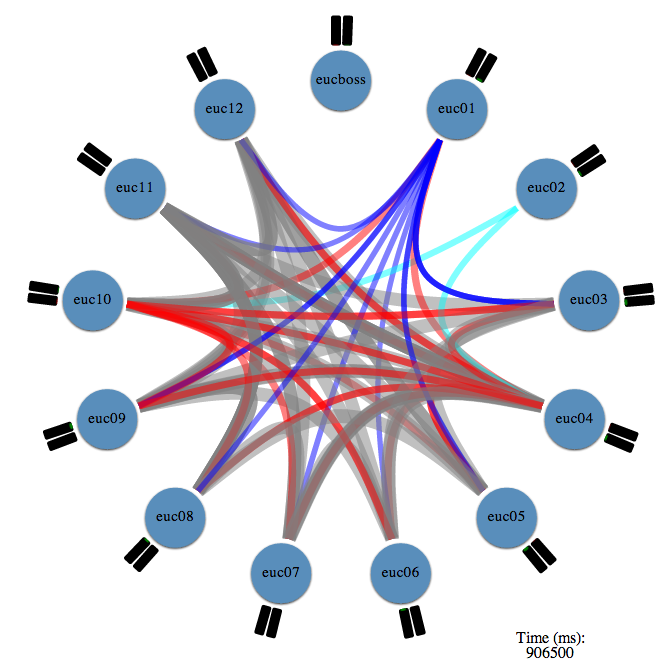
\includegraphics[width=0.6\textwidth]{figures/hadoop-viz.png}
\caption{Screenshot of visualization of Hadoop traffic, explained in Section~\ref{ssec:comp}.}
\label{fig:viz}
\end{figure}
